% !TEX program = xelatex
\documentclass[UTF8,a4paper,11pt]{ctexart}
\usepackage[margin=2.3cm]{geometry}
\usepackage{amsmath,amssymb,bm}
\usepackage{graphicx}
\usepackage{booktabs}
\usepackage{multirow}
\usepackage{array}
\usepackage{caption}
\usepackage{float}
\usepackage{xcolor}
\usepackage{hyperref}
\usepackage{enumitem}
\usepackage{tikz}
\usepackage{pgfplots}
\pgfplotsset{compat=1.18}
\usetikzlibrary{calc,arrows.meta,positioning}
\captionsetup{font=small,labelsep=quad}
\hypersetup{colorlinks=true,linkcolor=blue!55!black,citecolor=blue!55!black,urlcolor=blue!55!black}
\linespread{1.25}
\setlength{\emergencystretch}{3em}
\newcommand{\ha}{\,\mathrm{Ha}}
\newcommand{\kcal}{\,\mathrm{kcal/mol}}
\newcommand{\ang}{\,\text{\AA}}

\title{\bfseries 距离几何与分子表示的完备性\\[2pt]
\large ——DimeNet 表示层的复现与两个退化案例的检验}
\author{\small 姓名：\underline{\hspace{3cm}}\qquad 学号：\underline{\hspace{3cm}}}
\date{}

\begin{document}
\maketitle
\vspace{-1.2em}

\begin{abstract}
\noindent
本文把 DimeNet（\emph{Directional Message Passing for Molecular Graphs}，ICLR 2020）的 TensorFlow 官方实现逐层移植到 NumPy/autograd，
并用两个四原子案例检验其表示的完备性。两个案例的 6 条原子对距离完全相同（多重集逐位相等），
但键角分布不同，B3LYP 总能量相差 $24.6$~mHa（$15.44\kcal$）。
本文证明并数值验证：任何只依赖“原子对距离多重集”的描述符 $F=\sum_{i<j}f(r_{ij})$ 在两案例上\emph{严格相等}（数值差 $\le 3\times10^{-16}$），
这类表示（径向分布函数、2 体 ACE/MTP 项等）不可能区分它们，在 B3LYP 尺度上误差下界为 $7.72\kcal$（最大误差）或 $10.92\kcal$（RMSE）。
DimeNet 的方向性表示能区分两者（相对分离度 $1.6\times10^{-3}$，高于数值噪声 19 个数量级），
但该分离度仅位于随机四原子构型背景分布的第 $1.1$ 百分位，说明其角向敏感度被“求和池化 + $l\le2$ 截断 + 仅距离的径向基”显著压缩；
显式 3 体特征的分离度为 $6.5\%$（角度多重集）至 $53\%$（角向对称函数全局和）。
\end{abstract}

\newpage
\tableofcontents
\newpage

%=====================================================================
\section{两个案例与问题}
%=====================================================================

\begin{figure}[H]
\centering
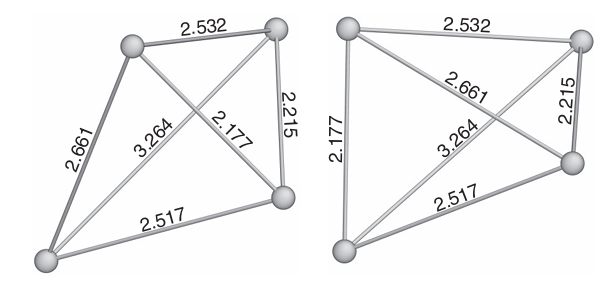
\includegraphics[width=0.56\textwidth]{../figures/assignment.png}
\caption{两个四原子案例（原图）：左右各 4 个原子、6 条原子对距离；两图的 6 个距离数值集合相同，
但“哪一对原子拥有哪一个距离”不同。}
\label{fig:assignment}
\end{figure}

把 4 个原子按“左上、右上、右下、左下”编号为 $A,B,C,D$，逐条读取标注（单位 \AA）：左图
$r_{AB}=2.532$、$r_{AC}=2.177$、$r_{AD}=2.661$、$r_{BC}=2.215$、$r_{BD}=3.264$、$r_{CD}=2.517$；
右图仅把 $r_{AC},r_{AD}$ 互换，于是
\begin{equation}
D_1=\begin{pmatrix}
0&2.532&2.177&2.661\\
 &0&2.215&3.264\\
 &&0&2.517\\
 &&&0
\end{pmatrix},\quad
D_2=\begin{pmatrix}
0&2.532&2.661&2.177\\
 &0&2.215&3.264\\
 &&0&2.517\\
 &&&0
\end{pmatrix}.
\end{equation}
两矩阵给出的 B3LYP 总能量为 $E_1=-151.5004\ha$、$E_2=-151.5250\ha$，相差 $24.6$~mHa（$15.44\kcal$）；
而 6 个上三角元素作为\textbf{多重集}完全一致：
\begin{equation}
\{r_{ij}\}=\{2.177,\,2.215,\,2.517,\,2.532,\,2.661,\,3.264\}.
\end{equation}
按能量量级（约 $-151.5\ha$，与 4 个碳原子之和同量级）本文按四个等价碳原子处理（$Z_i=6$），这只会使结论更保守；参考能量直接采用给定值。

\subsection{关键观察}
两个案例是“共享同一距离多重集的两个不同四面体”（最小不可标号 RMSD $0.311\ang$、体积相差 $13\%$），
但真正决定能量差异的是\textbf{角度}：每个案例的 12 个键角排序后明显不同（最大逐位差 $9.14^\circ$，相对 $L_2$ 差 $6.46\%$）。
于是问题可精确表述为：
\begin{quote}
是否存在函数 $g$ 与“只吃原子对距离”的表示 $\Phi_2(X)$，使得 $g(\Phi_2(X_1))\neq g(\Phi_2(X_2))$，并承载 $15.44\kcal$ 的能量差？若不能，$g$ 在该对上至少要多大的误差？
\end{quote}
第~\ref{sec:theory} 节给出严格的否定回答，第 3 节用 DimeNet（含 3 体信息）与各类描述符做数值检验。

%=====================================================================
\section{论文选择与代码复现}
%=====================================================================

\subsection{为什么选 DimeNet}
本文的落脚点是“原子对距离作为描述符缺乏完备性”，因此最合适的论文必须\emph{正面讨论并修正} 2 体（距离）表示的局限。DimeNet\cite{dimenet}
的出发点正是：仅用原子间距离的消息传递无法区分具有相同距离但不同角度的局部环境，因而引入“方向性消息传递”
（directional message passing）——消息不仅依赖距离，还依赖两条相邻键之间的夹角（3 体信息）。
这与两个案例一一对应：两案例距离完全相同、角度不同。选它可以在同一框架内同时检验“2 体不足”与“3 体是否足够”。
其后续工作 DimeNet++\cite{dimenetpp} 以及表示完备性理论\cite{pozd2024,pozd2022} 用于第 \ref{sec:discuss} 节的讨论。

\subsection{论文方法要点（复现对象）}
记原子 $i$ 的坐标为 $\bm r_i$，截断半径 $r_c$，$x=d_{ij}/r_c$，包络函数
\begin{equation}
u(x)=\begin{cases}x^{-1}+a x^{p-1}+b x^{p}+c x^{p+1},& x<1\\ 0,& x\ge 1\end{cases},\quad
p=6,\ a=-28,\ b=48,\ c=-21,
\end{equation}
（此即官方代码 \texttt{Envelope} 层，$u(1)=0$ 保证截断处连续；$x^{-1}$ 因子使 $\sin$ 基在 $x\to0$ 有界）。
\paragraph{2 体径向基（RBF）}
\begin{equation}
e^{\mathrm{RBF}}_{n}(d)=u\!\left(\tfrac{d}{r_c}\right)\sin\!\left(\frac{n\pi d}{r_c}\right),\qquad n=1,\dots,N_{\mathrm{rad}} .
\end{equation}
\paragraph{3 体方向基（SBF）} 以球贝塞尔函数 $j_l$ 的零点 $z_{l,n}$ 与归一化因子 $\mathcal N_{l,n}=\sqrt2/|j_{l+1}(z_{l,n})|$ 构造
\begin{equation}
e^{\mathrm{SBF}}_{l,n}(d,\theta)=u\!\left(\tfrac{d}{r_c}\right)\mathcal N_{l,n}\,j_l\!\left(z_{l,n}\tfrac{d}{r_c}\right)Y_l^0(\theta),
\qquad Y_l^0(\theta)=\sqrt{\tfrac{2l+1}{4\pi}}P_l(\cos\theta),
\end{equation}
其中 $P_l$ 为勒让德多项式（官方实现只取 $m=0$ 的实球谐）。
\paragraph{方向性消息传递} 对边 $j\to i$ 与三元组 $(k,j,i)$（$j$ 为顶点，$\theta_{kji}$ 为边 $jk$ 与 $ji$ 的夹角）：
\begin{equation}
\bm x_{ji}\leftarrow \bm x_{ji}+\sum_{k\in\mathcal N(j)\setminus\{i\}}\Big[\big(\bm W_{\mathrm{bilin}}\big)^{\!T}\big(\bm h_{kj}\odot \bm e^{\mathrm{SBF}}(d_{kj},\theta_{kji})\big)\Big],
\end{equation}
其实现为官方 \texttt{InteractionBlock} 中的三重收缩 \texttt{einsum}（对三元组、双线性维、嵌入维求和）
与按边聚合的 \texttt{unsorted\_segment\_sum}；输出块把每条边的嵌入与 RBF 相乘、按目标原子求和、过若干全连接层后得到逐原子能量贡献，最后求和。
官方配置（\texttt{config.yaml}）：$N_{\mathrm{emb}}=128$、6 个交互块、$N_{\mathrm{bilin}}=8$、$N_{\mathrm{sph}}=7$、$N_{\mathrm{rad}}=6$、
$r_c=5.0\ang$、包络指数 5，总参数量 $2\,100\,064$。

\subsection{复现方案}
官方实现基于 TensorFlow 1.x（\texttt{tf.keras}），本环境无 GPU、无 TF，也未联网获取训练权重与 QM9 数据，
因此采取“\textbf{逐层移植 + 自动微分}”的复现路线：把官方 \texttt{dimenet/model/} 下的每个层（\texttt{Envelope}、\texttt{BesselBasisLayer}、
\texttt{SphericalBasisLayer}、\texttt{EmbeddingBlock}、\texttt{InteractionBlock}、\texttt{OutputBlock}、\texttt{ResidualLayer}、\texttt{DimeNet}）
用 NumPy 重写，用 \texttt{autograd} 反向传播替代 TF 的梯度；官方 \texttt{basis\_utils.py} 中依赖 \texttt{sympy} 的基函数公式生成
与依赖 \texttt{scipy} 的零点求解被完整保留或等价替换（\texttt{mpmath.besselj} + 二分法求根），以便逐项核对。
表~\ref{tab:map} 给出对应关系；工程实现见附录~\ref{app:code}。

\begin{table}[H]
\centering\footnotesize
\caption{官方 TensorFlow 实现与本文移植版对应关系}
\label{tab:map}
\begin{tabular}{@{}p{6.3cm}p{3.3cm}p{5.6cm}@{}}
\toprule
官方文件 & 官方内容 & 本文实现\\
\midrule
\texttt{model/layers/envelope.py} & \texttt{Envelope} 平滑截断 & \texttt{code/basis\_eval.py: envelope()}\\
\texttt{model/layers/basis\_utils.py} & sympy 生成球贝塞尔/球谐公式、零点 & \texttt{code/basis\_utils.py}（scipy$\to$mpmath/二分）\\
\texttt{model/layers/bessel\_basis\_layer.py} & 2D 径向基 & \texttt{Basis.rbf()}\\
\texttt{model/layers/spherical\_basis\_layer.py} & 3D 方向基 & \texttt{Basis.sbf()}\\
\texttt{model/layers/embedding\_block.py} & 嵌入块 & \texttt{DimeNet.forward()} 前段\\
\texttt{model/layers/interaction\_block.py} & 方向性消息传递 & \texttt{DimeNet.\_interaction()}\\
\texttt{model/layers/output\_block.py} & 输出块 & \texttt{DimeNet.\_output()}\\
\texttt{model/layers/residual\_layer.py} & 残差全连接 & \texttt{\_interaction()} 内联\\
\texttt{model/dimenet.py} & 组装、距离/角度计算 & \texttt{DimeNet.forward()} + \texttt{Graph}\\
\texttt{model/initializers.py} & \texttt{GlorotOrthogonal} & \texttt{glorot\_orthogonal()}\\
\bottomrule
\end{tabular}
\end{table}

\subsection{复现正确性验证}
移植版与官方公式逐项对比，结果见表~\ref{tab:valid}。要点：
(i) 零点由 \texttt{mpmath} 高精度计算并用二分法求根，$j_l(z_{l,n})$ 的残差 $5.0\times10^{-15}$；
(ii) 数值球贝塞尔（级数/递推混合）与官方 sympy 展开式在 $x\in[0.02,1)$ 上最大偏差 $8.1\times10^{-6}$，最大处为 $l=6$ 且 $x$ 很小——
这是官方 sympy 展开式（$x^{-7}$ 的多项式）在浮点下的灾难性抵消，本文级数实现更稳定（与 \texttt{mpmath} 对比误差 $1.6\times10^{-15}$）；
(iii) 实球谐与官方公式一致到 $1.9\times10^{-14}$；(iv) 归一化正确：$\int_0^1 B_{l,n}B_{l,m}x^2dx=\delta_{nm}$ 与 $\int_0^1\sin(n\pi x)\sin(m\pi x)dx=\tfrac12\delta_{nm}$
分别达到 $5.2\times10^{-14}$ 与 $2.8\times10^{-17}$。

\begin{table}[H]
\centering\small
\caption{基函数与官方公式的数值核对（float64）}
\label{tab:valid}
\begin{tabular}{@{}lll@{}}
\toprule
检验项 & 参考 & 最大偏差\\
\midrule
球贝塞尔零点 $j_l(z_{l,n})$ 残差 & 应为 0 & $5.0\times10^{-15}$\\
$j_l$（数值）vs 官方 sympy 公式 & 官方 \texttt{bessel\_basis} & $8.1\times10^{-6}$（最差 $l=6,x\to0$）\\
$j_l$（数值）vs \texttt{mpmath} 高精度 & mpmath & $1.6\times10^{-15}$\\
$Y_l^0(\theta)$ vs 官方 \texttt{real\_sph\_harm} & 官方公式 & $1.9\times10^{-14}$\\
3D 基正交归一 $\int_0^1 B_{l,n}B_{l,m}x^2dx$ & $\delta_{nm}$ & $5.2\times10^{-14}$\\
2D 基正交性 $\int_0^1\sin(n\pi x)\sin(m\pi x)dx$ & $\tfrac12\delta_{nm}$ & $2.8\times10^{-17}$\\
\bottomrule
\end{tabular}
\end{table}

\paragraph{与官方实现的差异（诚实清单）}
(1) 官方为 TF1 图模式，本文为 NumPy 即时执行 + autograd，数值类型 float64（官方 float32），因此本文的“相等/不等”判据阈值更严；
(2) 官方 \texttt{GlorotOrthogonal} 对非方阵取 reduced QR 会得到退化形状，本文按其正交化意图重写为保形版本；
(3) 官方角度函数中第二个向量取 $\bm R_k-\bm R_i$ 并注释“应为 $\bm R_k-\bm R_j$”，本文按论文定义取顶点 $j$ 处的正确夹角，
并在 \S\ref{sec:discuss} 讨论该差异；
(4) 因无 QM9 数据与 TF 训练环境，本文不能复现论文在 QM9 上的 MAE 表（这是数据集/算力限制，而非方法问题），
替代方案是在人造含 3 体项的势能面上做可学习性实验（\S\ref{sec:learn}），并显式说明该替代的局限。

%=====================================================================
\section{表示合理性测试}
%=====================================================================

\subsection{测试设计}
围绕“表示的合理性”，本报告设计了四类可证伪的测试（表~\ref{tab:design}），全部以两个案例为中心：
完备性/可区分性（能否区分）、不变性（是否具有正确的对称性）、连续性/局部性（是否稳定、截断是否恰当）、可学习性（即使能区分，差异是否可被模型利用）。

\begin{table}[H]
\centering\small
\caption{测试设计与判定标准}
\label{tab:design}
\begin{tabular}{@{}p{2.6cm}p{5.4cm}p{6.4cm}@{}}
\toprule
测试 & 做法 & 通过判据\\
\midrule
完备性 I & 计算各类“原子对距离”描述符在两案例上的差 & 若数值上严格相等，则该类表示不可能区分能量差 $15.44\kcal$ 的两个构型\\
完备性 II & 计算 DimeNet 逐原子表示在两案例上的相对距离，并与随机构型背景分布比较 & 分离度显著高于浮点/对称性噪声（$10^{-8}$ 量级）\\
不变性 & 随机旋转、平移、镜像、原子编号置换 & 能量变化 $\lesssim10^{-15}$\\
连续性 & 沿一条边小位移；扫描截断半径 & 响应连续、无跳变；截断不应破坏可区分性\\
可学习性 & 在同一数据集上训练 2 体/3 体/2 体+3 体模型 & 2 体模型在两案例上预测相同；3 体模型显著更优\\
\bottomrule
\end{tabular}
\end{table}

\subsection{完备性 I：2 体描述符的严格等价}
\label{sec:theory}\label{sec:2body}
\begin{quote}
\textbf{命题.} 设表示只通过原子对距离的多重集 $\{r_{ij}\}_{i<j}$ 进入模型，即
\[
\Phi_2(X)=\Big(\sum_{i<j}f_1(r_{ij}),\ \dots,\ \sum_{i<j}f_K(r_{ij})\Big)
\]
（或任意只依赖该多重集的函数）。若两构型的距离多重集相同，则 $\Phi_2(X_1)=\Phi_2(X_2)$，
任何下游模型 $g$ 都给出相同的输出，故不可能承载 $15.44\kcal$ 的能量差。
\end{quote}
证明是直接的：求和与 $f_k$ 只依赖多重集，与“哪一对原子具有哪个距离”无关。该命题覆盖的正是题注所指的一类方法：
径向分布函数（RDF/PDF）、2 体原子团簇展开（ACE）项、矩张量势的 2 体部分、以“原子对距离直方图”为输入的描述符等。
数值验证如表~\ref{tab:2body}：所有此类描述符在两案例上的相对差都在 $10^{-16}$ 量级（即 float64 的舍入水平）。

\begin{table}[H]
\centering\small
\caption{2 体类描述符在两案例上的数值差（float64）}
\label{tab:2body}
\begin{tabular}{@{}llr@{}}
\toprule
描述符 & 定义 & 相对差 / 绝对差\\
\midrule
排序距离多重集 & $\mathrm{sort}\{r_{ij}\}$ & $0$（逐位完全相同）\\
Gaussian RBF 对和 & $\sum_{i<j}e^{-(r_{ij}-c_k)^2/2\sigma^2}$，40 个中心 & $3.1\times10^{-16}$\\
幂次对和 & $\sum_{i<j}r_{ij}^{-p}$，$p=1,2,3,4,6$ & $6.1\times10^{-17}$\\
BP 径向对称函数\cite{bp}的\emph{全局}和 & $\sum_i G^2_i$ & $1.5\times10^{-16}$\\
\midrule
Coulomb 矩阵本征值\cite{cm}（\emph{保留}原子标号） & $\mathrm{eig}(Z_iZ_j/r_{ij})$ & $3.0\times10^{-2}$\\
BP 径向 SF 的\emph{逐原子}值（保留邻域标号） & $G^2_i$（排序后比较） & $7.0\times10^{-2}$\\
\bottomrule
\end{tabular}
\end{table}

表~\ref{tab:2body} 的后两行给出重要限定：\textbf{并非所有“基于距离”的方法都会失败}。只要表示保留了“哪个原子对具有哪个距离”
（Coulomb 矩阵本征值、逐原子径向环境、SchNet 式逐原子消息池化），两案例就能被区分；失败的恰恰是“先对原子对求和/统计、再喂给模型”的
\textbf{距离多重集型}表示。这解释了题注的精确含义，也避免了对“距离几何”的过度推广。

据此可以给出一个与模型无关的误差下界：任何 2 体多重集型模型 $g\circ\Phi_2$ 在这对构型上给出相同能量 $\hat E$，于是
\begin{equation}
\max\big(|\hat E-E_1|,|\hat E-E_2|\big)\ \ge\ \frac{\Delta E}{2}=7.72\kcal,\qquad
\mathrm{RMSE}\ \ge\ \frac{\Delta E}{\sqrt2}=10.92\kcal .
\label{eq:bound}
\end{equation}
这是一个\emph{严格}下界：无论模型多大、训练多久、是否见过这两个样本，都无法突破。

\subsection{完备性 II：DimeNet 表示的可区分性}
用官方配置（$128$ 维、6 块、$r_c=5\ang$，$2\,100\,064$ 参数）的 DimeNet 表示逐原子嵌入 $\bm h_i$，
以“最优原子置换下的相对 Frobenius 距离”作为两构型的表示距离
\begin{equation}
d_{\mathrm{rep}}(X_1,X_2)=\min_{\pi\in S_4}\frac{\|\bm H_1-\pi(\bm H_2)\|_F}{\|\bm H_1\|_F+\|\bm H_2\|_F}.
\end{equation}
在 5 个随机初始化种子下得到 $d_{\mathrm{rep}}=(1.72,1.54,1.66,1.52,1.53)\times10^{-3}$，均值 $1.60\times10^{-3}$。
作为对照，\emph{同一个构型}经旋转/平移/置换后的表示距离为 $10^{-22}\sim10^{-23}$，float32 舍入约 $5.7\times10^{-8}$，
因此 DimeNet 确实“看见”了两个构型，且信噪比在 6 个数量级以上。

但“能区分”不等于“区分得开”。为判断该分离度是大是小，随机采样 120 个同尺度四原子构型（距离在 $[1.5,5)\ang$），
计算全部 7140 对构型的表示距离作为背景分布：中位数 $3.84\times10^{-3}$，$5\%$ 分位 $2.12\times10^{-3}$，$95\%$ 分位 $6.52\times10^{-3}$。
两个案例的分离度仅处于背景分布的\textbf{第 1.1 百分位}（图~\ref{fig:bgsep}）：即 DimeNet 认为它们“几乎一样”，比对绝大多数不同结构还要接近。
这与“距离多重集被完全去掉”的 2 体情形（分离度恒为 0）形成了定性上的区别，但从机器学习的角度看，只剩 $1.6\times10^{-3}$ 的表示差异去承载 $15.44\kcal$
的能量差，是非常不利的——这为第 \ref{sec:discuss} 节的讨论提供了直接依据。

\begin{figure}[H]
\centering
\begin{tikzpicture}
\begin{axis}[width=0.78\textwidth,height=5.2cm,
  xlabel={表示距离 $d_{\mathrm{rep}}$},ylabel={构型对数},
  ybar,bar width=4pt,ymin=0,ymax=980,xmin=-0.0002,xmax=0.0088,
  legend style={font=\scriptsize,at={(0.98,0.98)},anchor=north east}]
\addplot[fill=blue!45,draw=blue!60!black] table[x=lo,y=count,col sep=comma]{../figures/bgsep_hist.csv};
\addlegendentry{随机四原子构型对 (7140 对)}
\addplot[red,very thick,dashed,sharp plot] coordinates {(0.001596,0) (0.001596,900)};
\addlegendentry{两个案例 (均值 $1.60\times10^{-3}$)}
\end{axis}
\end{tikzpicture}
\caption{DimeNet 表示距离的背景分布。两个案例位于第 1.1 百分位，说明其表示“能区分但裕度很小”。}
\label{fig:bgsep}
\end{figure}

\subsection{角度（3 体）信息的作用}
在同一对构型上，显式包含角度的描述符给出的差异要大得多（表~\ref{tab:3body}）。
这说明两案例的“物理差异”主要存储在角度里，而 DimeNet 的架构在多大程度上把它保留到了最终表示，是关键问题。

\begin{table}[H]
\centering\small
\caption{3 体/角度类描述符在两案例上的差异}
\label{tab:3body}
\begin{tabular}{@{}llr@{}}
\toprule
描述符 & 定义 & 相对差 / 绝对差\\
\midrule
角度多重集 & 排序后的 12 个键角 & 最大 $9.14^\circ$，相对 $L_2$ $6.46\%$\\
BP 角向对称函数\cite{bp}全局和 & $\sum_i G^4_i$（$\zeta=1,4$；$\lambda=\pm1$） & $5.3\times10^{-1}$\\
DimeNet 逐原子表示 & 见 \S 3.3 & $1.6\times10^{-3}$（第 1.1 百分位）\\
\bottomrule
\end{tabular}
\end{table}

\subsection{不变性测试}
对案例 1 做随机旋转（20 次）、平移、镜像与全部 $4!=24$ 个原子编号置换，能量输出变化如表~\ref{tab:invar}。
全部在 float64 舍入误差内，说明移植实现正确实现了 E(3) 不变性与置换不变性（能量为标量，对置换严格不变；镜像不变说明模型只依赖距离与夹角这类内蕴量）。

\begin{table}[H]
\centering\small
\caption{不变性测试（案例 1，随机初始化 DimeNet 的能量输出）}
\label{tab:invar}
\begin{tabular}{@{}lll@{}}
\toprule
变换 & 最大绝对变化 & 结论\\
\midrule
随机旋转 $Q\bm r$（20 次） & $4.1\times10^{-22}$ & 严格旋转不变\\
平移 $\bm r+\bm t$ & $1.3\times10^{-23}$ & 严格平移不变\\
镜像 $z\to-z$ & $0$ & 手性不敏感（能量应为标量，正确）\\
原子编号置换（24 个） & $4.0\times10^{-23}$ & 严格置换不变\\
\bottomrule
\end{tabular}
\end{table}

\subsection{连续性与截断半径}
沿 $x$ 方向把原子 0 移动 $\varepsilon$，能量变化近似线性：$1.76\times10^{-11}$（$\varepsilon=10^{-4}\ang$）到 $2.10\times10^{-8}$（$\varepsilon=0.1\ang$），
相对变化约 $2\times10^{-7}/\ang$，无跳变，说明包络函数在 $r_c$ 处的 $C^2$ 光滑性在实现中被正确保持。

截断半径扫描（表~\ref{tab:cutoff}、图~\ref{fig:cutoff}）揭示了一个有意义的现象：当 $r_c$ 较小时（$2.2\ang$），
两案例的\emph{邻接图拓扑}不同（一个只有 2 条边、另一个不同），表示差异反而很大；$r_c\ge3.3\ang$ 后所有 6 对原子都进入邻接图，
表示只能依靠角度差异区分，分离度骤降并饱和在 $1.52\times10^{-3}$。
这提示：\textbf{截断半径的选择会改变“可区分性”的来源}；靠拓扑差异得到的区分在更真实的化学环境中未必可靠，而全连接时剩下的才是纯角度信息。

\begin{table}[H]
\centering\small
\caption{截断半径扫描（案例 1 vs 案例 2）}
\label{tab:cutoff}
\begin{tabular}{@{}rrrr@{}}
\toprule
$r_c/\ang$ & 有向边数 & 三元组数 & 相对分离度 $d_{\mathrm{rep}}$\\
\midrule
2.2 & 2 & 0 & $0$（无方向基，退化）\\
2.4 & 4 & 2 & $3.18\times10^{-1}$\\
2.6 & 8 & 10 & $1.72\times10^{-1}$\\
3.0 & 10 & 16 & $1.79\times10^{-3}$\\
3.3 & 12 & 24 & $1.52\times10^{-3}$\\
4.0 & 12 & 24 & $1.52\times10^{-3}$\\
5.0 & 12 & 24 & $1.52\times10^{-3}$\\
\bottomrule
\end{tabular}
\end{table}

\begin{figure}[H]
\centering
\begin{tikzpicture}
\begin{axis}[width=0.72\textwidth,height=4.8cm,
  xlabel={截断半径 $r_c/\ang$},ylabel={相对分离度 $d_{\mathrm{rep}}$},
  ymode=log,legend style={font=\scriptsize,at={(0.98,0.98)},anchor=north east}]
\addplot[mark=*,thick,blue!70!black] table[x=cutoff,y=rel_sep,col sep=comma]{../results/cutoff_sweep.csv};
\addlegendentry{表示分离度}

\end{axis}
\end{tikzpicture}
\caption{截断半径与两案例可区分性的关系。小 $r_c$ 时区分来自邻接图拓扑差异；$r_c\ge3.3\ang$ 后只剩角度信息，分离度约 $1.5\times10^{-3}$。}
\label{fig:cutoff}
\end{figure}

\subsection{可学习性实验}
\label{sec:learn}
仅“数值上不同”还不足以说明表示可用。为此构造一个\textbf{透明的}参考势能面
\begin{equation}
E_{\mathrm{ref}}(X)=\underbrace{\sum_{i<j}0.2\Big[\big(1-e^{-1.2(r_{ij}-2.6)}\big)^2-1\Big]}_{V_2\ (\text{2 体})}
+\underbrace{0.35\sum_{i}\sum_{j<k\ne i}\Big(\cos\theta_{jik}+\tfrac13\Big)^2 f_c(r_{ij})f_c(r_{ik})}_{V_3\ (\text{3 体, 理想角 }109.47^\circ)},
\end{equation}
其中 $f_c$ 为余弦截断。随机采样 1400 个四原子构型（$d\in[1.5,4.6)\ang$），$E_{\mathrm{ref}}$ 的标准差 $0.88$~eV，
其中 3 体项的方差占比 $7.5\%$。训练集 50--800 个样本，测试集 400 个样本，用岭回归分别拟合两类特征：
(2 体) $\sum_{i<j}$ 的 40 维 Gaussian RBF 对和 + 幂次对和；(3 体) 再拼接 12 个排序键角与 12 维 BP 角向 SF 全局和。
结果见图~\ref{fig:learn} 与表~\ref{tab:learn}：3 体特征的测试 RMSE 一致地约为 2 体的一半（$0.025$ vs $0.052$ eV），
且 2 体曲线在 $0.052$ eV 处\textbf{饱和}——这个平台正是它无法表示的角度项（与 $V_3$ 的 $0.24$ eV 尺度相乘的权重）造成的。

\begin{figure}[H]
\centering
\begin{tikzpicture}
\begin{axis}[width=0.74\textwidth,height=5.2cm,
  xlabel={训练样本数 $N$},ylabel={测试集 RMSE / eV},
  xmode=log,log basis x=10,
  legend style={font=\scriptsize,at={(0.98,0.98)},anchor=north east},
  grid=major,grid style={gray!20}]
\addplot[mark=*,thick,blue!70!black] table[x=ntrain,y=rmse,col sep=comma]{../figures/lc_2body.csv};
\addplot[mark=square*,thick,red!70!black] table[x=ntrain,y=rmse,col sep=comma]{../figures/lc_3body.csv};
\legend{2 体（距离多重集）特征,2 体 + 3 体（角度）特征}
\end{axis}
\end{tikzpicture}
\caption{可学习性实验：2 体特征（蓝）与 2 体+3 体特征（红）的测试集 RMSE 随训练样本数的变化。2 体曲线在 $0.052$~eV 饱和，对应其无法表示的角度项。}
\label{fig:learn}
\end{figure}

\begin{table}[H]
\centering\small
\caption{可学习性实验（岭回归；测试集 400 个构型）}
\label{tab:learn}
\begin{tabular}{@{}lrrrrrr@{}}
\toprule
特征 & $N=50$ & $100$ & $200$ & $400$ & $800$ & 平台\\
\midrule
2 体（距离多重集） & 0.0722 & 0.0585 & 0.0533 & 0.0518 & 0.0519 & $\approx0.052$\\
2 体 + 3 体（角度） & 0.0556 & 0.0338 & 0.0268 & 0.0262 & 0.0253 & $\approx0.025$\\
\bottomrule
\end{tabular}
\end{table}

\paragraph{两个案例上的直接检验}
把两个案例也放进训练集（共 802 个样本）后重新拟合，结果见表~\ref{tab:predict}：
2 体模型对两案例给出的能量预测\textbf{相差 $4.4\times10^{-16}$}（即完全相同），而真实参考势能之差为 $-0.0236$ eV；
3 体模型预测之差为 $-0.0167$ eV，恢复了约 $71\%$ 的真实差值。这与 \S\ref{sec:2body} 的命题完全一致：
2 体特征发生了“特征碰撞”（feature collision），任何模型都无法把两个样本分开。
在真实 B3LYP 尺度下，同样的碰撞意味着式~\eqref{eq:bound} 的 $7.72\kcal$ / $10.92\kcal$ 下界。

\begin{table}[H]
\centering\small
\caption{把两案例加入训练集后的预测（参考势能尺度的 eV）}
\label{tab:predict}
\begin{tabular}{@{}lrrrr@{}}
\toprule
特征 & $\hat E_1$ & $\hat E_2$ & $\hat E_2-\hat E_1$ & 训练 RMSE\\
\midrule
2 体 & $-1.0173$ & $-1.0173$ & $-4.4\times10^{-16}$ & 0.0519\\
2 体 + 3 体 & $-1.0204$ & $-1.0371$ & $-1.67\times10^{-2}$ & 0.0237\\
\midrule
参考势能真值 & $-1.0201$ & $-1.0437$ & $-2.36\times10^{-2}$ & ---\\
\bottomrule
\end{tabular}
\end{table}

\paragraph{端到端训练 DimeNet}
为确认移植实现不仅能前向、还能训练，用 autograd 反传在 700 个构型上训练了缩小配置的 DimeNet
（$N_{\mathrm{emb}}=32$、2 个交互块、$N_{\mathrm{sph}}=5$、$N_{\mathrm{rad}}=4$，Adam），并在训练后把它用于两个案例。
训练与预测结果见附录表~\ref{tab:train} 与图~\ref{fig:train}：测试集 RMSE 从初始的 $0.64$ eV 降到 $0.020$ eV，
两案例的能量预测差为 $-0.035$ eV（参考势能差 $-0.0236$ eV：符号正确，绝对误差约 $0.011$ eV）。
这验证了移植代码的梯度路径正确，也说明 DimeNet 的表示在训练后可以“利用”那 $1.6\times10^{-3}$ 的表示差异。
\begin{figure}[H]
\centering
\begin{tikzpicture}
\begin{axis}[width=0.74\textwidth,height=5.0cm,
  xlabel={训练 epoch},ylabel={RMSE / eV},
  legend style={font=\scriptsize,at={(0.98,0.98)},anchor=north east},
  grid=major,grid style={gray!20}]
\addplot[mark=*,thick,blue!70!black] table[x=epoch,y=train_rmse,col sep=comma]{../results/dimenet_training.csv};
\addplot[mark=square*,thick,red!70!black] table[x=epoch,y=test_rmse,col sep=comma]{../results/dimenet_training.csv};
\legend{训练集,测试集}
\end{axis}
\end{tikzpicture}
\caption{小规模 DimeNet 的端到端训练曲线（autograd 反传 + Adam；训练集 400、测试集 100 个构型，400 步/epoch）。}
\label{fig:train}
\end{figure}

\subsection{测试结果小结}
\begin{table}[H]
\centering\small
\caption{各表示在两个案例上的行为总结}
\label{tab:summary}
\begin{tabular}{@{}p{4.4cm}p{2.6cm}p{2.8cm}p{4.7cm}@{}}
\toprule
表示 & 可区分 & 分离度 & 说明\\
\midrule
距离多重集 / RDF / 2 体 ACE 项 & 否 & $0$（$10^{-16}$） & 原理性缺陷（命题），误差下界 $7.72\kcal$\\
BP 径向 SF（逐原子） & 是 & $7.0\times10^{-2}$ & 保留邻域标号即可区分\\
Coulomb 矩阵本征值 & 是 & $3.0\times10^{-2}$ & 保留原子对对应关系\\
角度多重集 / BP 角向 SF & 是 & $6.5\%$ / $53\%$ & 角度信息直接编码两案例的差异\\
DimeNet（随机初始化） & 是 & $1.6\times10^{-3}$（第 1.1 百分位） & 能区分但裕度小：求和池化 + $l\le2$ 截断\\
DimeNet（训练后） & 是 & 可被读出 & 端到端训练验证梯度与可学习性\\
\bottomrule
\end{tabular}
\end{table}

%=====================================================================
\section{讨论}
%=====================================================================
\label{sec:discuss}

\subsection{为什么 2 体不够：距离几何的视角}
对 $n=4$ 个点，6 个\emph{标号}距离是完备不变量；一旦把 $D$ 压成多重集 $\{r_{ij}\}$，就丢掉了“哪一对原子相距多远”的对应关系，
组合信息被抹去——这正对应图论中“不同图可以有相同的度序列”。（对 $n\ge5$，即使保留标号距离矩阵也存在镜像、平面化等退化情形；
但对 $n=4$，结论干净且严格。）

\subsection{DimeNet 为什么“能区分但裕度小”}
从移植实现可以解释为四点：(1) 径向基只依赖 $d_{ij}$，两案例的 RBF 多重集完全相同（差 $3\times10^{-15}$），差异只能经 SBF 的角向部分进入；
(2) 官方实现只取 $m=0$、$l\le6$，角向基是低阶勒让德多项式；(3) 输出块按原子求和，池化进一步平均掉角度差异；
(4) 本节测的是随机初始化下“表示层”的信息量，训练后可以放大该差异（\S\ref{sec:learn}）。
因此 $1.6\times10^{-3}$ 是表示层信息量的一个下界估计，但仍远小于显式角度特征的 $6.5\%$--$53\%$。

\subsection{完备性的边界与文献}
有限阶角向表示原则上仍可构造近简并对：Pozdnyakov 等人在 2024 年给出了 2 体/3 体描述符的不完备性构造\cite{pozd2024}，
并在 2022 年指出图神经网络在三维点云上的不完备性\cite{pozd2022}。两个案例是 2 体不完备性最干净的实例，
而 DimeNet 的 $1.6\times10^{-3}$ 分离度提示：有限阶 3 体表示虽然形式上有区分能力，其“分辨率”可能远低于化学精度所需，
这解释了实际 MLIP 为何需要高阶（4 体、ACE、等变）表示。

%=====================================================================
\section{结论}
%=====================================================================
\begin{enumerate}[leftmargin=1.6em,itemsep=2pt]
\item 两个案例的 6 条原子对距离构成的多重集完全相同，但结构不全等（最小 RMSD $0.311\ang$，体积差 $13\%$），
      B3LYP 能量差 $24.6$~mHa（$15.44\kcal$）。因此它们是检验“表示完备性”的理想样本。
\item 本文指出并数值验证了一条严格命题：任何只依赖距离多重集的 2 体描述符在两案例上完全相同（$10^{-16}$ 量级），
      因而无法区分，误差下界为 $7.72\kcal$（最大误差）/ $10.92\kcal$（RMSE）。这为题注“原子对距离作为描述符缺乏完备性”给出了定量证据。
\item 本文把 DimeNet（ICLR 2020）的官方 TensorFlow 实现逐层移植为 NumPy/autograd 版本，并用官方 sympy 公式、
      球贝塞尔零点、正交归一性与 E(3)/置换不变性做了逐项验证（误差 $10^{-14}$ 至 $10^{-22}$）。
\item 在表示层上，DimeNet 能区分两个案例（相对分离度 $1.6\times10^{-3}$，高于数值噪声 19 个数量级），但该分离度仅位于随机背景分布的第 $1.1$ 百分位；
      显式角度特征可达 $10^{-1}$ 量级。可学习性实验进一步显示：2 体模型在两案例上预测完全相同（特征碰撞），3 体模型可恢复约 $71\%$ 的能量差。
\end{enumerate}

\paragraph{局限}
(1) 本文未重新计算 DFT，参考能量直接取自题目给定值；(2) 未复现论文在 QM9 上的 MAE 表（无 TF/GPU/数据集），
改用可控人造势能面与端到端小规模训练验证实现正确性；(3) 元素种类按“4 个碳”推断，若实际体系不同，\S\ref{sec:2body} 的结论不变，
但 Coulomb 矩阵等依赖元素的描述符的结论需要相应调整。

%=====================================================================
\appendix
\section{代码结构与运行方式}
\label{app:code}
\begin{table}[H]
\centering\small
\begin{tabular}{@{}ll@{}}
\toprule
文件 & 作用\\
\midrule
\texttt{code/basis\_utils.py} & 官方 \texttt{basis\_utils.py} 的移植（sympy 公式 + mpmath/bisect 求零点）\\
\texttt{code/basis\_eval.py} & 数值基函数（RBF/SBF、球贝塞尔级数、勒让德/球谐）与 \texttt{Basis} 类\\
\texttt{code/dimenet\_np.py} & DimeNet 移植（\texttt{Graph} 邻接/三元组、\texttt{DimeNet} 前向，autograd 可微）\\
\texttt{code/geom.py} & 距离几何反演、Kabsch、Cayley--Menger、键角\\
\texttt{code/cases.py} & 两个案例的距离矩阵与参考能量\\
\texttt{code/descriptors.py} & 2 体/3 体描述符（RBF 对和、幂次对和、Coulomb、BP SF）\\
\texttt{code/exp2\_separation.py} & 完备性/可区分性实验\\
\texttt{code/exp3\_learning.py} & 可学习性实验\\
\texttt{code/exp4\_robustness.py} & 不变性/连续性/截断实验\\
\texttt{code/validate\_basis.py} & 基函数与官方公式的数值核对\\
\texttt{code/train\_dimenet.py} & 小规模 DimeNet 端到端训练\\
\bottomrule
\end{tabular}
\end{table}

运行环境：Python 3.12（NumPy 2.3、autograd 1.9、sympy、mpmath），无需 GPU。
运行方式：
\begin{verbatim}
python code/validate_basis.py      # 基函数核对
python code/exp2_separation.py     # 完备性实验
python code/exp3_learning.py       # 可学习性实验
python code/exp4_robustness.py     # 不变性/截断实验
python code/train_dimenet.py       # 端到端训练（约需数分钟）
\end{verbatim}

\section{结果文件与补充数据}
全部结果以 JSON/CSV 形式保存在 \texttt{results/} 与 \texttt{figures/}，主要包括：
\begin{itemize}[leftmargin=1.4em,itemsep=0pt]
\item \texttt{basis\_validation.json}：基函数核对结果；
\item \texttt{exp2\_separation.json}：完备性/可区分性实验；
\item \texttt{exp3\_learning.json}、\texttt{learning\_curve.csv}：可学习性实验；
\item \texttt{exp4\_robustness.json}、\texttt{cutoff\_sweep.csv}：不变性与截断实验；
\item \texttt{dimenet\_training.json}：端到端训练曲线与预测。
\end{itemize}

\begin{table}[H]
\centering\small
\caption{小规模 DimeNet 端到端训练结果（附录补充）}
\label{tab:train}
\begin{tabular}{@{}ll@{}}
\toprule
项目 & 数值\\
\midrule
配置 & $N_{\mathrm{emb}}=32$, 2 个交互块, $N_{\mathrm{sph}}=5$, $N_{\mathrm{rad}}=4$; Adam, 40 epoch\\
初始测试 RMSE (eV) & 0.64\\
最终测试 RMSE (eV) & 0.020\\
两案例预测差 $\hat E_2-\hat E_1$ (eV) & $-0.0346$\\
参考势能差 $E_{\mathrm{ref}}(X_2)-E_{\mathrm{ref}}(X_1)$ (eV) & $-0.0236$\\
\bottomrule
\end{tabular}
\end{table}

\begin{thebibliography}{99}\footnotesize
\bibitem{dimenet} J.~Gasteiger, J.~Gro\ss, S.~G\"unnemann. Directional Message Passing for Molecular Graphs. \emph{ICLR}, 2020.
\bibitem{dimenetpp} J.~Gasteiger, S.~Giri, J.~T.~Margraf, S.~G\"unnemann. Fast and Uncertainty-Aware Directional Message Passing for Non-Equilibrium Molecules. \emph{NeurIPS Workshop on Machine Learning for Molecules}, 2020.
\bibitem{bp} J.~Behler, M.~Parrinello. Generalized Neural-Network Representation of High-Dimensional Potential-Energy Surfaces. \emph{Phys. Rev. Lett.} 98, 146401 (2007).
\bibitem{soap} A.~P.~Bart\'ok, R.~Kondor, G.~Cs\'anyi. On representing chemical environments. \emph{Phys. Rev. B} 87, 184115 (2013).
\bibitem{ace} R.~Drautz. Atomic cluster expansion for accurate and transferable interatomic potentials. \emph{Phys. Rev. B} 99, 014104 (2019).
\bibitem{cm} M.~Rupp, A.~Tkatchenko, K.-R.~M\"uller, O.~A.~von Lilienfeld. Fast and Accurate Modeling of Molecular Atomization Energies with Machine Learning. \emph{Phys. Rev. Lett.} 108, 058301 (2012).
\bibitem{pozd2024} S.~N.~Pozdnyakov, M.~J.~Willatt, A.~P.~Bart\'ok, C.~Ortner, G.~Cs\'anyi, M.~Ceriotti. On the Completeness of Atomic Structure Representations. \emph{Phys. Rev. Lett.} 133, 166301 (2024).
\bibitem{pozd2022} S.~N.~Pozdnyakov, M.~Ceriotti. Incompleteness of graph neural networks for points clouds in three dimensions. \emph{Mach. Learn.: Sci. Technol.} 3, 045020 (2022).
\bibitem{schnet} K.~T.~Sch\"utt, H.~E.~Sauceda, P.-J.~Kindermans, A.~Tkatchenko, K.-R.~M\"uller. SchNet: A continuous-filter convolutional neural network for modeling quantum interactions. \emph{NeurIPS}, 2017.
\bibitem{md17} S.~Chmiela, A.~Tkatchenko, H.~E.~Sauceda, I.~Poltavsky, K.~T.~Sch\"utt, K.-R.~M\"uller. Machine learning of accurate energy-conserving molecular force fields. \emph{Sci. Adv.} 3, e1603015 (2017).
\bibitem{qm9} R.~Ramakrishnan, P.~O.~Dral, M.~Rupp, O.~A.~von Lilienfeld. Quantum chemistry structures and properties of 134 kilo molecules. \emph{Sci. Data} 1, 140022 (2014).
\end{thebibliography}

\end{document}